\chapter{Resultate}
%
In diesem Kapitel werden ausgewählte Messergebnisse vorgeführt. Zu Beginn werden einige Plots präsentiert, die für die Auswertung verwendet wurden. Anschließend werden Unterschiede zwischen den Ergebnissen aufgezeigt, die im nächsten Kapitel für die Evaluierung der Methoden diskutiert werden. Alle Messungen wurden ohne Störungen oder Fehler von außerhalb erfolgreich durchgeführt.\\
Die nachfolgende Tab. \ref{tab:tabelle4} zeigt zu jeder Testperson die vorab ermittelte Ruhe-\gls{HF}, die während der Leistungsdiagnostik \gls{HFmax} sowie die \gls{Wstart}, die \gls{Wmax} und die \acrfull{VO2max}. 16 von 28 Personen mussten die Belastungsphase laut eigener Aussage wegen Beinschwäche beenden. Zehn Probanden erreichten nach Selbsteinschätzung ihr konditionales Maximum. Zwei Personen klagten in der letzten Stufe über Atemnot und mussten den Test deshalb abbrechen.
%
\begin{table}[H]
	\centering
		\caption{Originäre Messergebnisse der Tests}
		\medskip
		\begin{tabulary}{\textwidth}{L C C C C C}
			\toprule
			ID & Ruhe-\gls{HF} in \si{\per\minute} & \gls{HFmax} in \si{\per\minute} & \gls{Wstart} in \si{\watt} & \gls{Wmax} in \si{\watt} & \gls{VO2max} in \si{\litre\per\minute} \\
			\midrule
			\midrule
			1w & 65 & 175 & 40 & 215 & 2,4 \\
			2w & 63 & 183 & 35 & 185 & 2,1 \\
			3w & 53 & 158 & 50 & 225 & 2,7 \\
			4m & 49 & 164 & 50 & 300 & 3,6 \\
			5w & 85 & 187 & 40 & 165 & 2,15 \\
			6w & 65 & 178 & 30 & 205 & 2,55 \\
			7m & 78 & 176 & 55 & 280 & 3,3 \\
			8m & 76 & 195 & 90 & 315 & 4 \\
			9m & 64 & 181 & 40 & 340 & 4,05 \\
			10w & 62 & 168 & 40 & 215 & 2,78 \\
			11m & 90 & 178 & 40 & 215 & 2,6 \\
			12m & 61 & 180 & 75 & 325 & 4 \\
			13m & 62 & 176 & 75 & 275 & 3,45 \\
			14m & 63 & 179 & 100 & 325 & 3,85 \\
			15m & 87 & 193 & 80 & 330 & 4,05 \\
			16w & 84 & 198 & 40 & 240 & 2,98 \\
			17w & 78 & 194 & 50 & 175 & 2 \\
			18w & 68 & 182 & 50 & 225 & 2,7 \\
			19w & 66 & 172 & 40 & 165 & 2,13 \\
			20m & 68 & 197 & 60 & 210 & 2,83 \\
			21m & 92 & 195 & 50 & 275 & 3,4 \\
			22m & 72 & 159 & 50 & 225 & 3,05 \\
			23w & 67 & 173 & 40 & 265 & 3,18 \\
			24m & 94 & 174 & 50 & 250 & 2,83 \\
			25m & 62 & 167 & 50 & 250 & 3,15 \\
			26m & 77 & 169 & 60 & 285 & 3,5 \\
			27m & 86 & 193 & 60 & 285 & 3,58 \\
			28w & 78 & 220 & 40 & 190 & 2,5 \\
			\bottomrule
		\end{tabulary}
		\label{tab:tabelle4}
\end{table}
%
\section{Grafiken zur Bestimmung der Schwellen}
%
\subsection{Manuelle Bestimmung}
%
\begin{figure}[H]
	\centering
	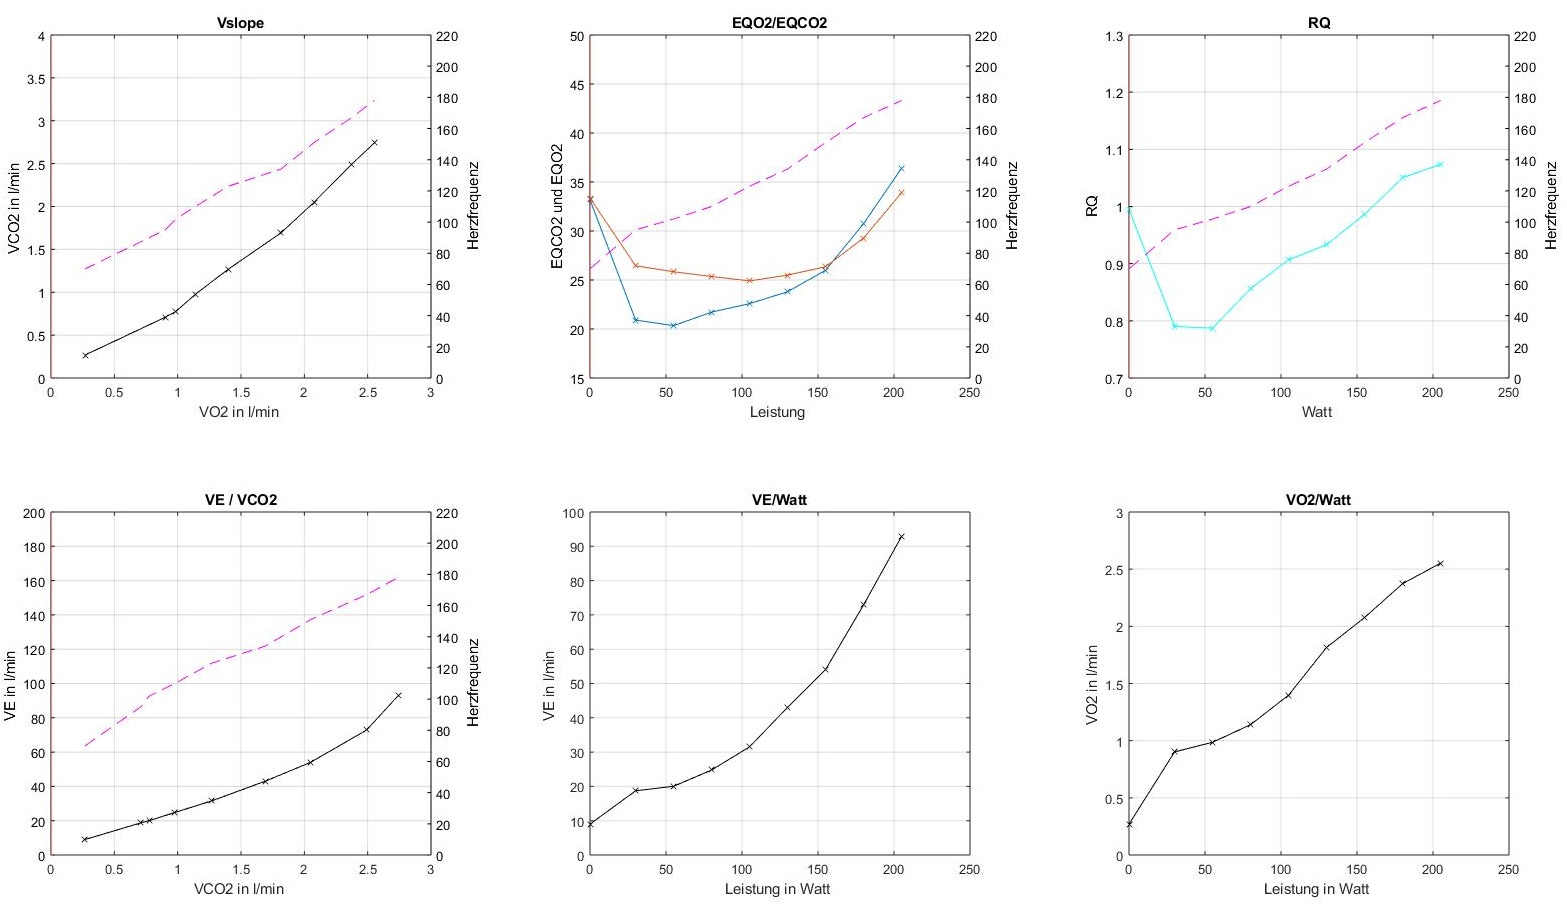
\includegraphics[width=\textwidth]{Bilder/plot_6w.jpg}
	\caption[6-Felder-Grafik von Probandin 6w]{6-Felder-Grafik von Probandin 6w; Feld 1: \gls{VCO2} in \si{\litre\per\minute} gegenüber der \gls{VO2} in \si{\litre\per\minute}; Feld 2: \gls{EQO2} in blau und \gls{EQCO2} in orange gegenüber der Leistung in \si{\watt}; Feld 3: \gls{RQ} gegenüber der Leistung in \si{\watt}; Feld 4: \gls{VE} in \si{\litre\per\minute} gegenüber der \gls{VCO2} in \si{\litre\per\minute}; Feld 5: \gls{VE} in \si{\litre\per\minute} gegenüber der Leistung in \si{\watt}; Feld 6: \gls{VO2} in \si{\litre\per\minute} gegenüber der Leistung in \si{\watt}; rosa gestrichelte Linie in Feld 1-4: \gls{HF} in \si{\per\minute}}
	\label{pic:pic15}
\end{figure}
%
Beginnend mit Abb. \ref{pic:pic15} für Probandin 6w werden beispielhaft Grafiken verschiedener Probanden vorgestellt, anhand derer die ventilatorischen Schwellen von den menschlichen Ratern subjektiv bestimmt wurden. Sie bestehen insgesamt aus sechs Feldern. Die ersten vier Felder stellen jeweils eine Methode zur Bestimmung der Schwellen dar. Sie enthalten zur erleichterten optischen Auswertung den Verlauf der \gls{HF} als rosafarbenen gestrichelten Graphen. Je nach Skalierung der Achsen, nimmt diese unterschiedliche Formen an und dient nur zum Vergleich mit den Graphen in demselben Feld. Sie wird durch die rechte Y-Achse skaliert. In Feld 5 und 6 werden die \gls{VE} sowie \gls{VO2} mit der Leistung (hier als "`Watt"' bezeichnet) in Relation gesetzt. Diese Plots wurden erstellt, um den Messungserfolg evaluieren zu können. Die Kreuze in den Kurven stellen die Mittelwerte einer Stufe dar und spiegeln in ihrer Menge die Anzahl der gefahrenen Belastungsstufen wider.
%
\begin{figure}[H]
	\centering
	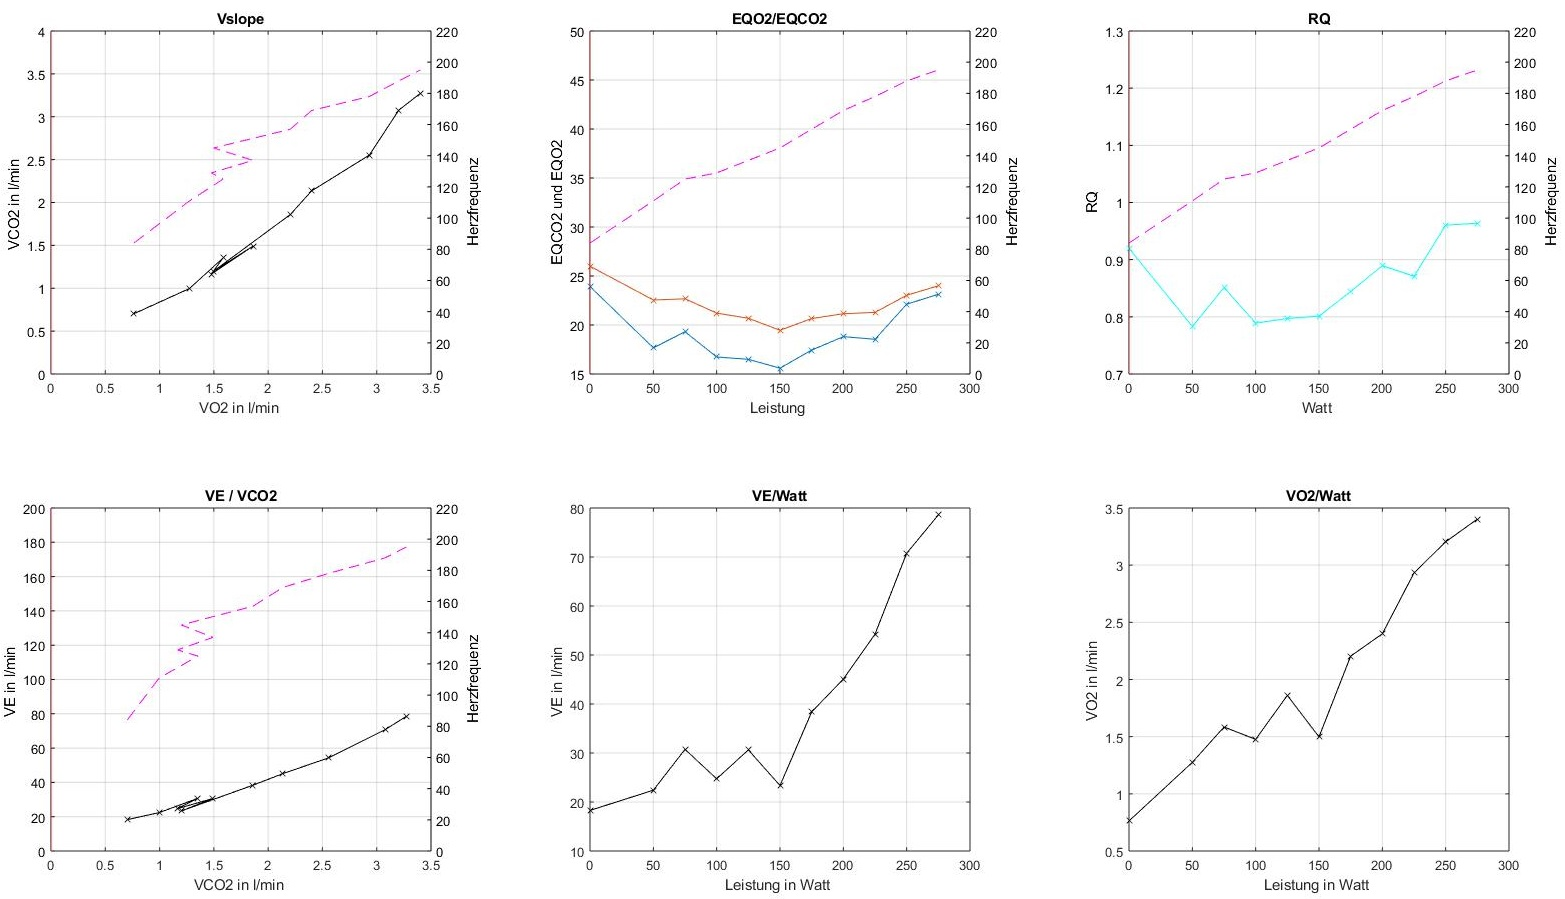
\includegraphics[width=\textwidth]{Bilder/plot_21m.jpg}
	\caption[6-Felder-Grafik von Proband 21m]{6-Felder-Grafik von Proband 21m; Feld 1: \gls{VCO2} in \si{\litre\per\minute} gegenüber der \gls{VO2} in \si{\litre\per\minute}; Feld 2: \gls{EQO2} in blau und \gls{EQCO2} in orange gegenüber der Leistung in \si{\watt}; Feld 3: \gls{RQ} gegenüber der Leistung in \si{\watt}; Feld 4: \gls{VE} in \si{\litre\per\minute} gegenüber der \gls{VCO2} in \si{\litre\per\minute}; Feld 5: \gls{VE} in \si{\litre\per\minute} gegenüber der Leistung in \si{\watt}; Feld 6: \gls{VO2} in \si{\litre\per\minute} gegenüber der Leistung in \si{\watt}; rosa gestrichelte Linie in Feld 1-4: \gls{HF} in \si{\per\minute}}
	\label{pic:pic16}
\end{figure}
%
Abb. \ref{pic:pic16} zeigt eine weitere 6-Felder-Grafik von Proband 21m. Diese beinhaltet unregelmäßige Graphen und es ist zu sehen, dass der RQ (hellblau) während des Tests den Wert eins nicht überschritten hat. Außerdem tritt in der \gls{EQCO2}-Kurve kein signifikanter Anstieg zum Ende der Leistungsdiagnostik auf. Die Graphen im 5. und 6. Feld besitzen in Abb. \ref{pic:pic15} stetige Steigungen. In Abb. \ref{pic:pic16} schwanken die Kurven zwischen einzelnen Messpunkten. Die übrigen Plots weisen an den betroffenen Stufen Analogien zu diesen Schwankungen auf. In Kapitel 4 werden diese Eigenschaften genauer erörtert.
%
\subsection{Algorithmische Bestimmung}
%
In diesem Abschnitt werden weitere Grafiken präsentiert, die zusätzlich eine algorithmische Schwellenbestimmung des MATLAB-Programms enthalten. Hierdurch wurde für jeden Probanden eine zweite Bilddatei erstellt, welche die VT1 und VT2 bereits in Form von vertikalen Linien beinhaltet und durch eine Angabe für die \gls{HF} an der jeweiligen Schwelle ergänzt ist. In Feld 5 dieser Plots wurde im Vergleich mit der \gls{VE} die Leistung durch die \gls{HF} ersetzt und es wurden bereits Trainingsbereiche eingefügt, die ebenfalls durch farbige vertikale Linien gekennzeichnet und in einer Legende mit Wertebereichen beschrieben sind. Es werden \gls{REKOM}, \gls{GA1}, \gls{GA2}, \gls{EW} und Leistung als Trainingszonen definiert. Dies diente dem Testlauf eines neuen Modells zur Trainingssteuerung. Die Entwicklung und Implementierung dieses Modells basierte auf den Erkenntnissen zur Schwellenbestimmung und wurde nachträglich eingefügt. Im Kapitel 5 wird näher darauf eingegangen.
%
\begin{figure}[H]
	\centering
	\noindent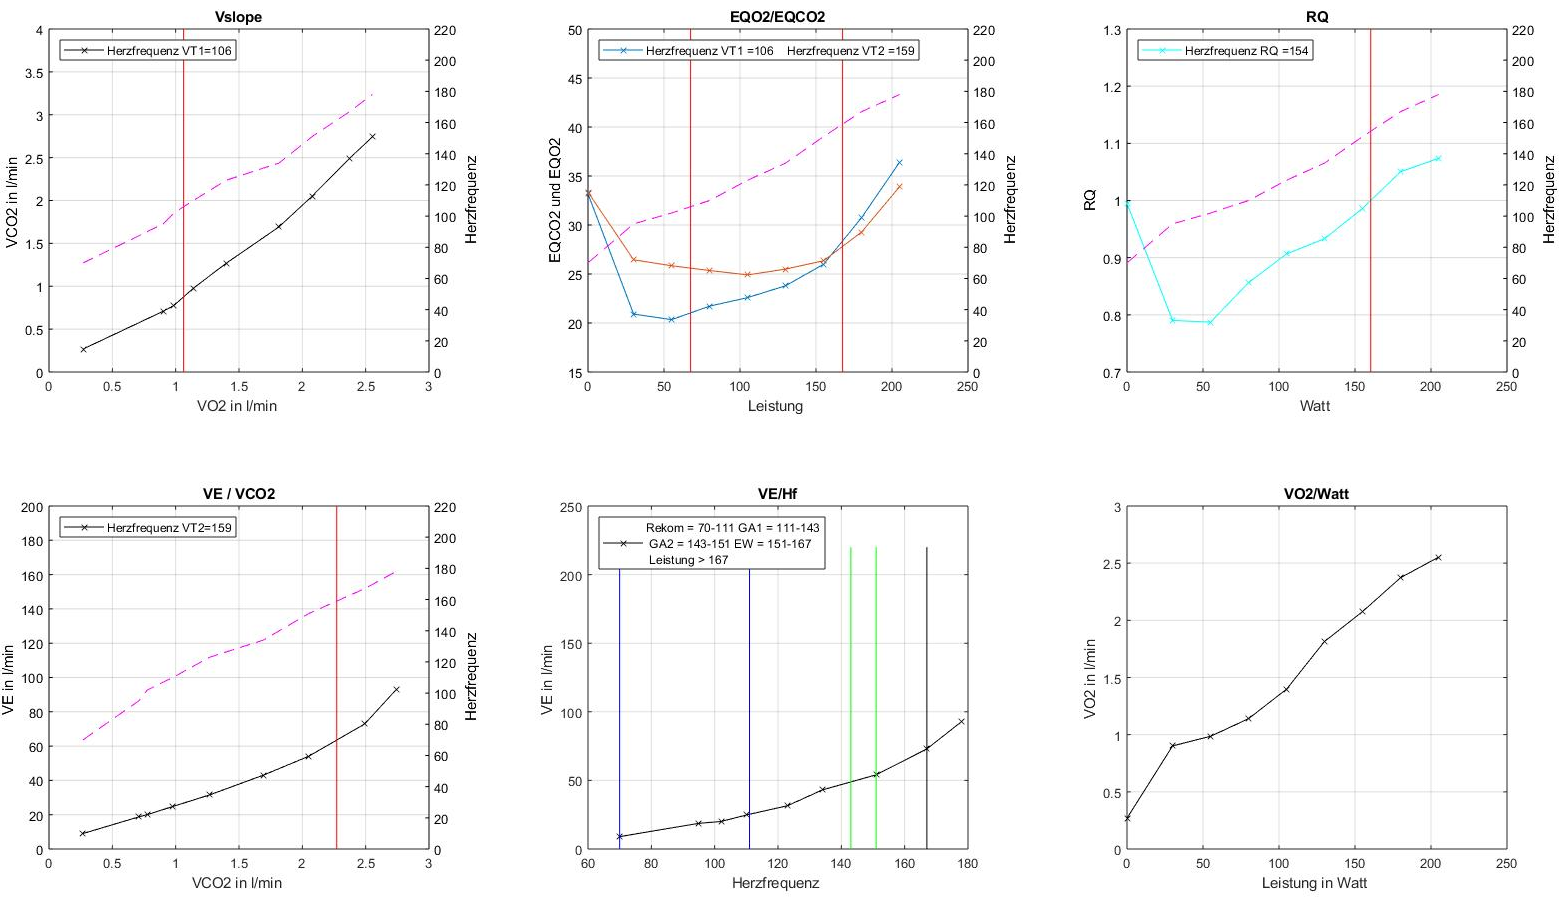
\includegraphics[angle=0,width=\linewidth,keepaspectratio]{Bilder/auto_6}
	\caption[6-Felder-Grafik von Probandin 6w mit algorithmischen Schwellenmarkierungen]{6-Felder-Grafik von Probandin 6w mit algorithmischen Schwellenmarkierungen in Form vertikaler roter Linien: \textsl{V-Slope} = \SI{106}{\per\minute}, \textsl{\gls{EQO2}} = \SI{106}{\per\minute}, \textsl{\gls{EQCO2}} = \SI{159}{\per\minute}, \textsl{\gls{VE}/\gls{VCO2}} = \SI{159}{\per\minute}\\Feld 5: \gls{VE} in \si{\litre\per\minute} gegenüber der \gls{HF} in \si{\per\minute} mit eingefügten Trainingszonen \gls{REKOM}, \gls{GA1}, \gls{GA2}, \gls{EW} und Leistung, abgegrenzt durch vertikale farbige Linien}
	\label{pic:pic17}
\end{figure}
%
Die Plots in Abb. \ref{pic:pic17} zeigen die detektierten Schwellen für Probandin 6w nach acht Stufen, bei der jeweils beide Methoden für die VT1 sowie VT2 identische Ergebnisse brachten. Im blauen \gls{EQO2}-Graphen ist zu sehen, dass VT1 zwischen Tiefpunkt und darauffolgendem Messpunkt bestimmt wurde. Am \gls{EQCO2} ist erkennbar, dass die VT2 beim ersten signifikanten Kurvenanstieg markiert wurde. Bei der Probandin stieg in der 7. Stufe der RQ über eins hinaus. Die mithilfe dieser Methode erhobene VT2 liegt bei einer \gls{HF} von \SI{154}{\per\minute}.
%
\begin{figure}[H]
	\centering
	\noindent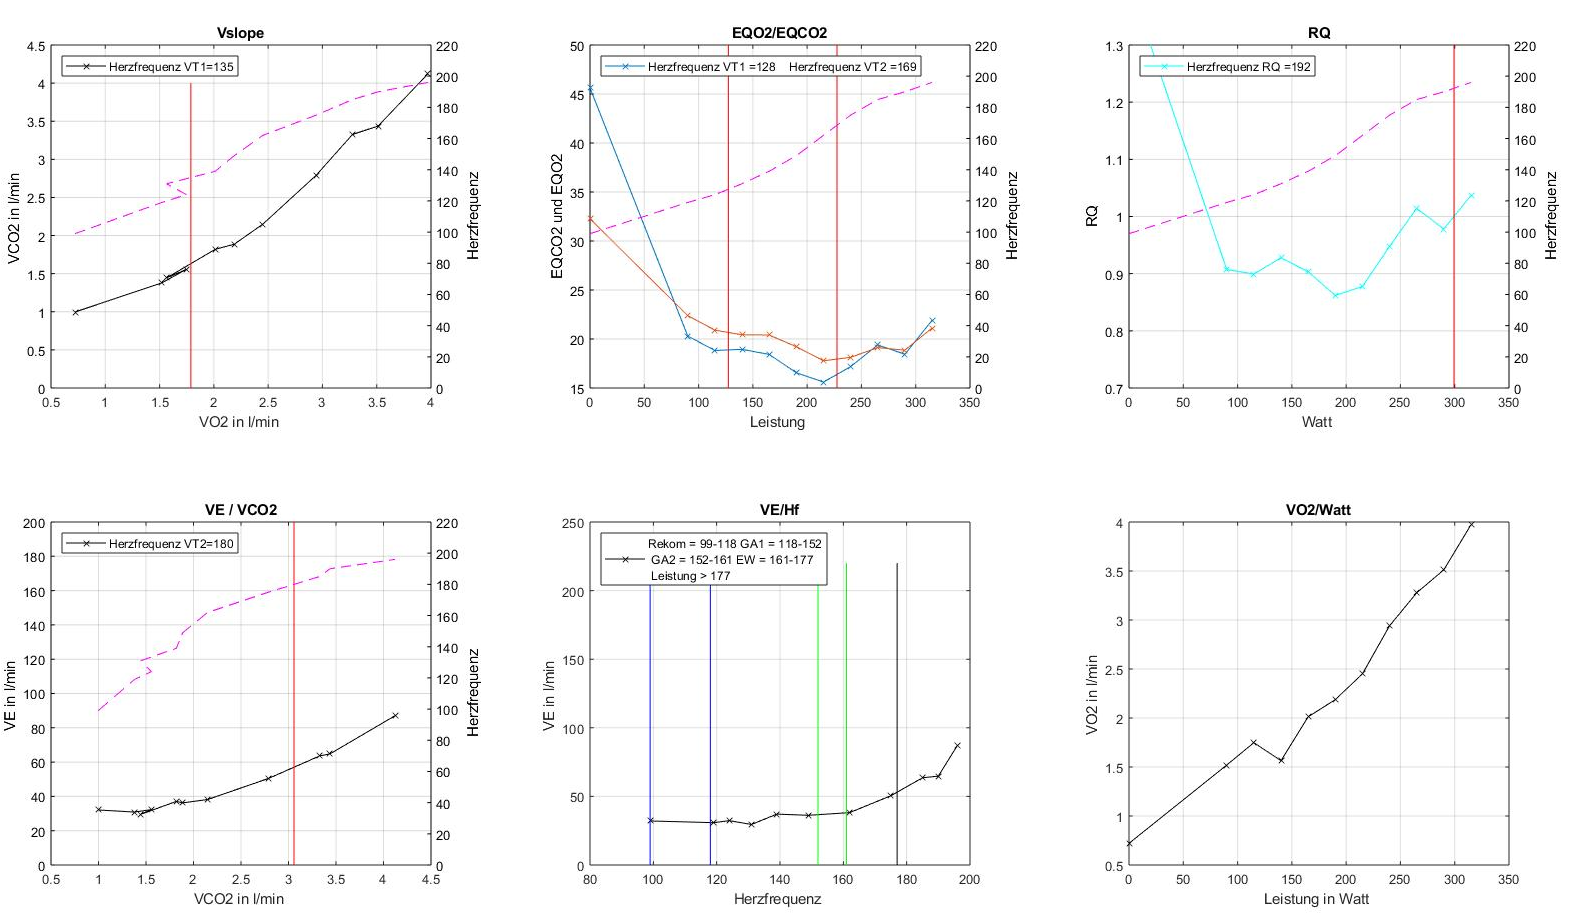
\includegraphics[angle=0,width=\linewidth,keepaspectratio]{Bilder/auto_8}
	\caption[6-Felder-Grafik von Proband 8m mit algorithmischen Schwellenmarkierungen]{6-Felder-Grafik von Proband 8m mit algorithmischen Schwellenmarkierungen: \textsl{V-Slope} = \SI{135}{\per\minute}, \textsl{\gls{EQO2}} = \SI{126}{\per\minute}, \textsl{\gls{EQCO2}} = \SI{169}{\per\minute}, \textsl{\gls{VE}/\gls{VCO2}} = \SI{180}{\per\minute}}
	\label{pic:pic18}
\end{figure}
%
In Abb. \ref{pic:pic18} ist die Grafik für Proband 8m erkennbar. Die \gls{HF} und der V-Slope in Feld 1 sowie \gls{VE}/\gls{VCO2} in Feld 4 sind zwischen Stufe 2 und 4 nicht differenzierbar. Die \gls{VO2} fällt im 6. Feld zwischen diesen Stufen. Der RQ schwankt zwischen den letzten zwei Messungen um den Wert eins herum und die Software bestimmte den zweiten Anstieg über eins bei \SI{192}{\per\minute} als VT2.\\
Abb. \ref{pic:pic19} stellt das Ergebnis von Proband 9m dar, der sogar 13 Belastungsstufen bewältigte. Mit RQ~=~1 wurde in der letzten Stufe bei \SI{173}{\per\minute} die VT2 markiert. In Feld 5 und 6 sind Schwankungen im Anstieg der \gls{VE} und \gls{VO2} in Relation zur \gls{HF} bzw. Belastung erkennbar.
%
\begin{figure}[H]
	\centering
	\noindent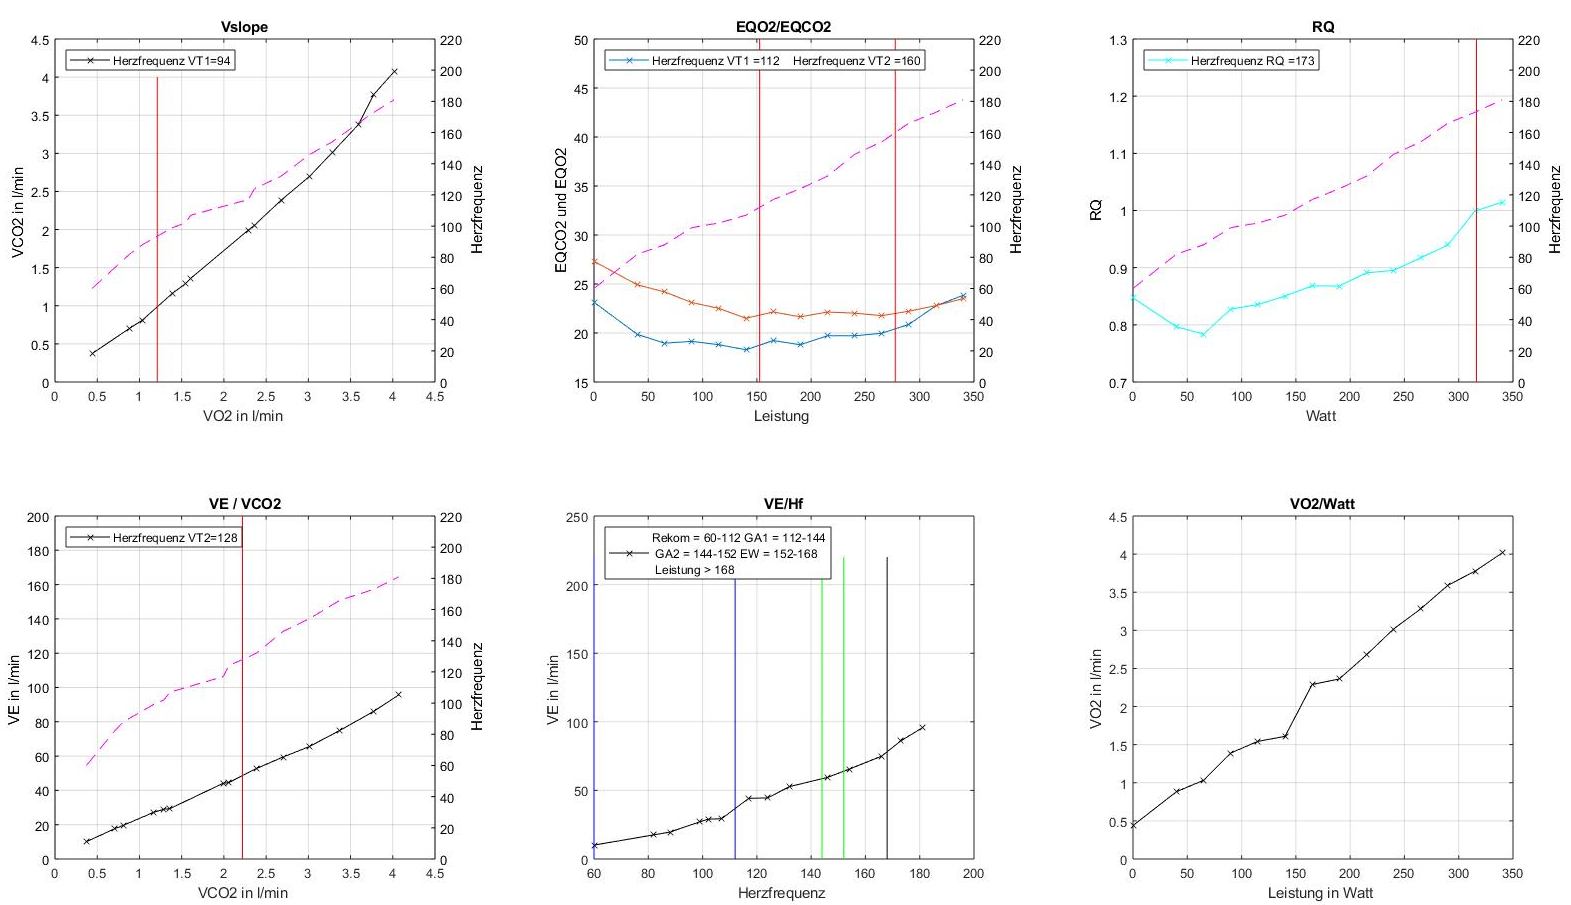
\includegraphics[angle=0,width=\linewidth,keepaspectratio]{Bilder/auto_9}
	\caption[6-Felder-Grafik von Proband 9m mit algorithmischen Schwellenmarkierungen]{6-Felder-Grafik von Proband 9m mit algorithmischen Schwellenmarkierungen: \textsl{V-Slope} = \SI{94}{\per\minute}, \textsl{\gls{EQO2}} = \SI{112}{\per\minute}, \textsl{\gls{EQCO2}} = \SI{160}{\per\minute}, \textsl{\gls{VE}/\gls{VCO2}} = \SI{128}{\per\minute}}
	\label{pic:pic19}
\end{figure}
%
\begin{figure}[H]
	\centering
	\noindent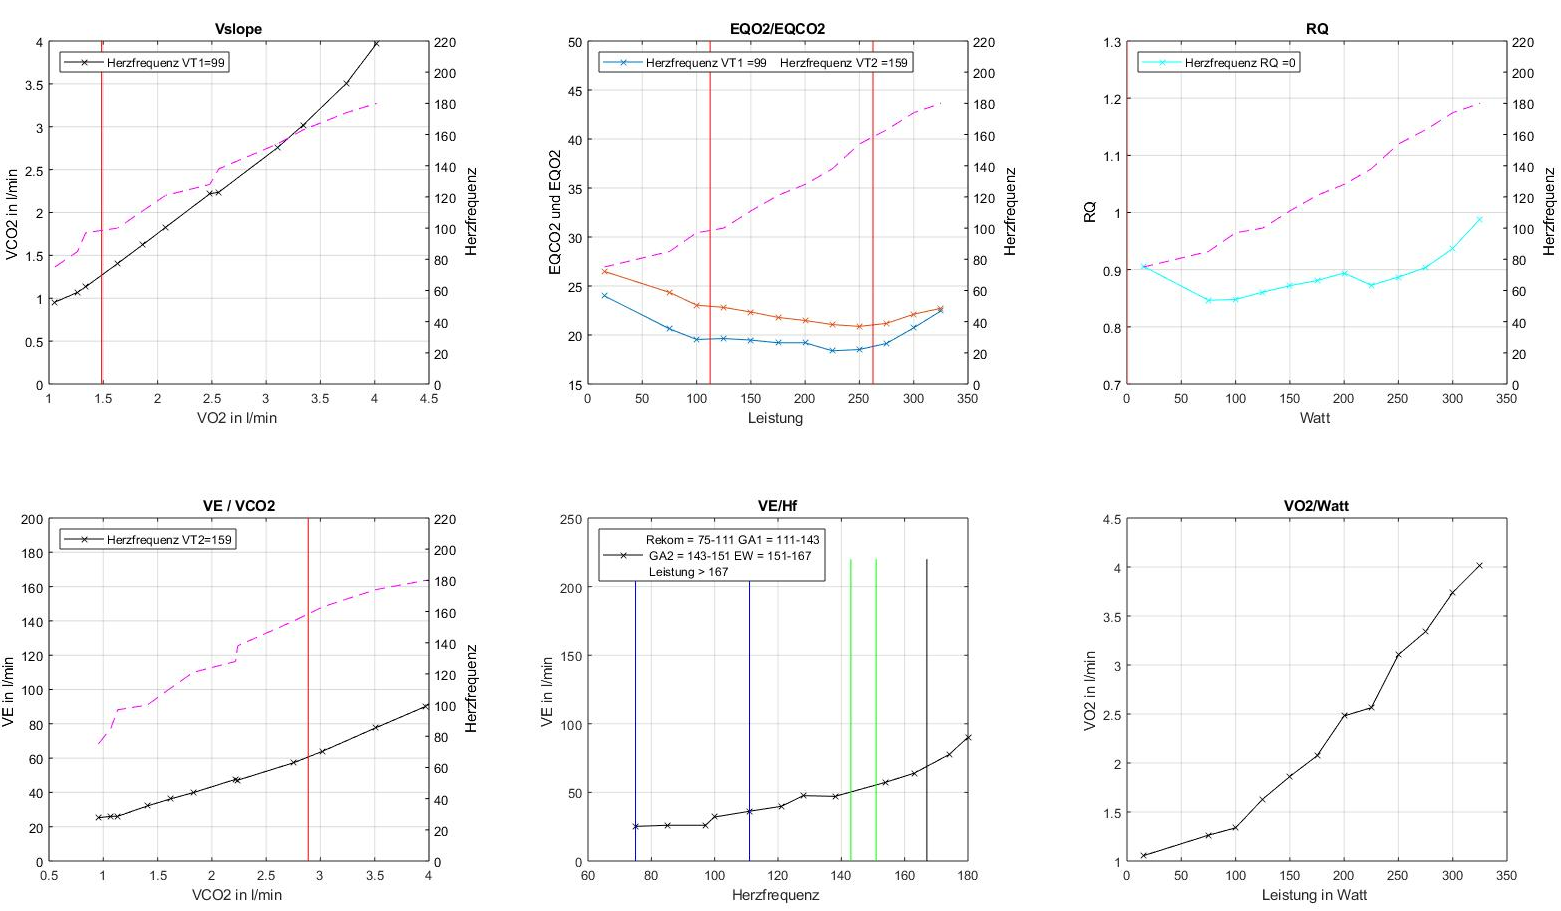
\includegraphics[angle=0,width=\linewidth,keepaspectratio]{Bilder/auto_12}
	\caption[6-Felder-Grafik von Proband 12m mit algorithmischen Schwellenmarkierungen]{6-Felder-Grafik von Proband 12m mit algorithmischen Schwellenmarkierungen: \textsl{V-Slope} = \SI{99}{\per\minute}, \textsl{\gls{EQO2}} = \SI{99}{\per\minute}, \textsl{\gls{EQCO2}} = \SI{159}{\per\minute}, \textsl{\gls{VE}/\gls{VCO2}} = \SI{159}{\per\minute}}
	\label{pic:pic20}
\end{figure}
%
In Abb. \ref{pic:pic20} ist eine Auswertung für Proband 12m zu sehen, welcher wiederum insgesamt elf Belastungsstufen absolvierte. Hier wurden die VT1 und VT2 ebenfalls mit beiden jeweiligen Methoden gleich bestimmt. Der RQ in Feld 3 stieg nicht über eins. Da die VT2 durch diese Methode vom Algorithmus nicht bestimmt werden konnte, ist der Wert null in der Legende angegeben. Im V-Slope sind mehrere Knickpunkte zu erkennen. Im 2. Feld tritt der Tiefpunkt des \gls{EQO2} erst in der 7. Stufe auf. Das \gls{EQCO2} sinkt an diesem Punkt noch, steigt jedoch ab der nächsten Stufe an. Im \gls{VO2}/Watt-Vergleich ist ein Knickpunkt mit geringerer Steigung ebenfalls nach der 7. Stufe zu sehen.
%
\begin{figure}[H]
	\centering
	\noindent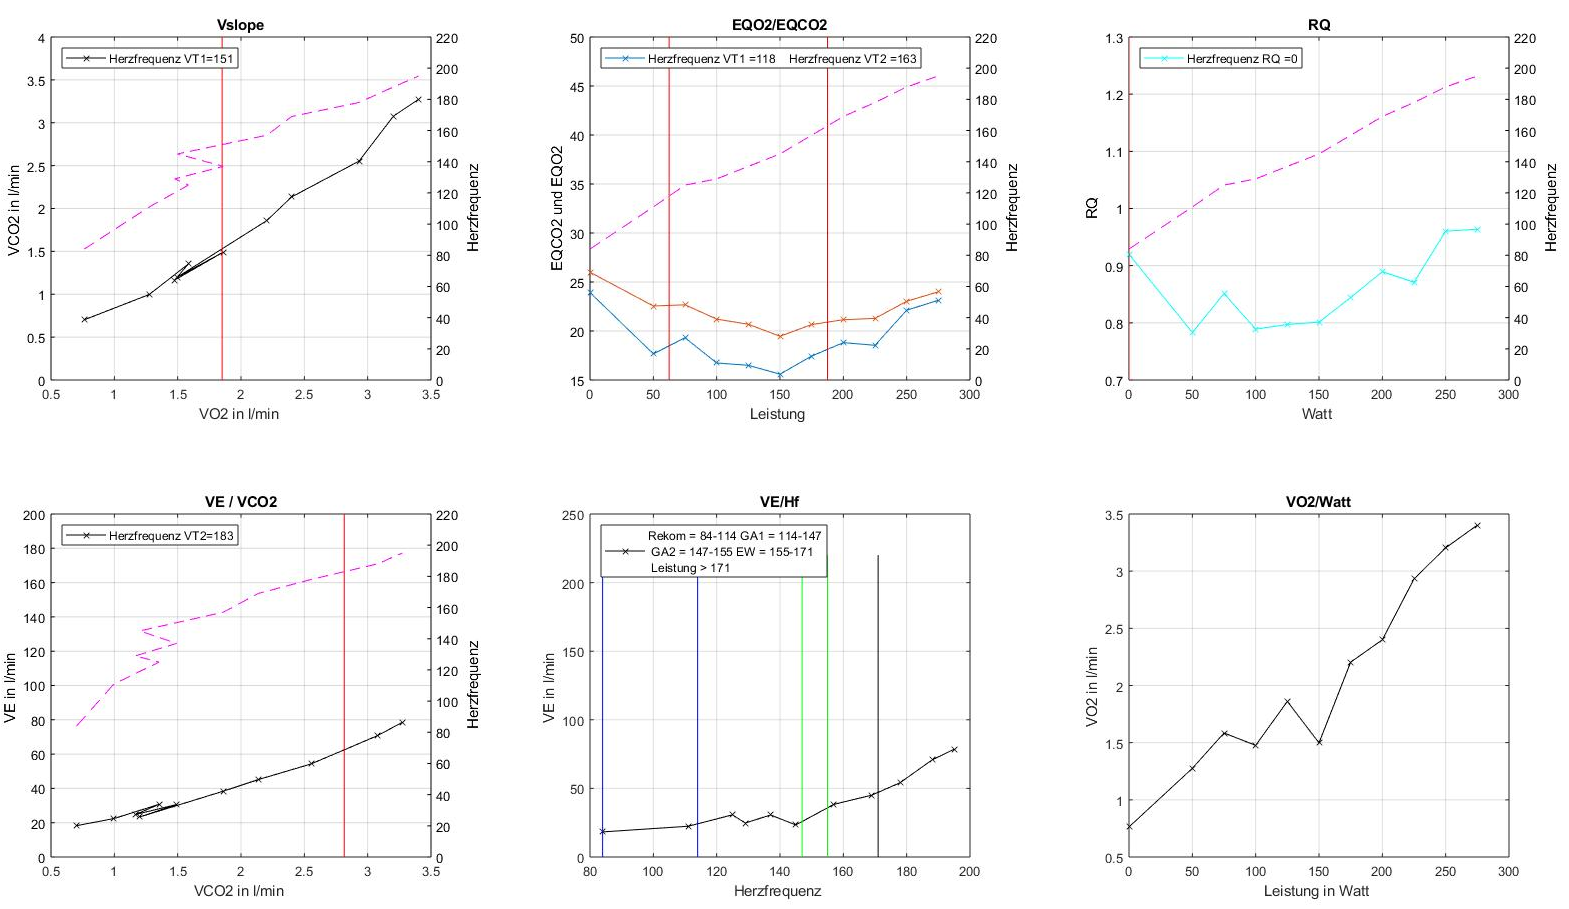
\includegraphics[angle=0,width=\linewidth,keepaspectratio]{Bilder/auto_21}
	\caption[6-Felder-Grafik von Proband 21m mit algorithmischen Schwellenmarkierungen]{6-Felder-Grafik von Proband 21m mit algorithmischen Schwellenmarkierungen: \textsl{V-Slope} = \SI{151}{\per\minute}, \textsl{\gls{EQO2}} = \SI{118}{\per\minute}, \textsl{\gls{EQCO2}} = \SI{163}{\per\minute}, \textsl{\gls{VE}/\gls{VCO2}} = \SI{183}{\per\minute}}
	\label{pic:pic21}
\end{figure}
%
Die vierte Beispielgrafik in Abb. \ref{pic:pic21} zeigt die Ergebnisse des Probanden 21m analog zu Abb. \ref{pic:pic16} inklusive der Schwellenbestimmung der Software. Dieser Proband bewältigte zehn Belastungsstufen. Im 6. Feld ist eine schwankende Steigung der \gls{VO2} in Relation zur Belastung zwischen Stufe 2 und 5 erkennbar. Diese Schwankungen tauchen auch im V-Slope und bei \gls{VE}/\gls{VCO2} sowie beim RQ auf. Auch hier unterscheiden sich die Bestimmungen für die VT1 durch den V-Slope und das \gls{EQO2} sowie jene für die VT2 anhand des \gls{EQCO2} oder \gls{VE}/\gls{VCO2}. Wie bereits in Abschnitt 3.3.1 erwähnt, erreichte der RQ dieses Probanden nicht den Wert eins.
%
\section{Ergebnisse der Schwellenbestimmung}
%
\subsection{Ergebnisse für die VT1}
%
\begin{table}[H]
	\begin{center}
		\caption{Ergebnisse für die \gls{HF} in \si{\per\minute} bei der VT1}
		\medskip
		\begin{tabulary}{\textwidth}{L@{\hspace{3em}} C C C C C C}
			\toprule
			& \multicolumn{2}{c}{\textbf{Rater 1}} & \multicolumn{2}{c}{\textbf{Rater 2}} & \multicolumn{2}{c}{\textbf{Software}} \\
			\midrule
			ID & V-Slope & \gls{EQO2} & V-Slope & \gls{EQO2} & V-Slope & \gls{EQO2} \\
			\midrule
			\midrule
			1w & 109 & 133 & 133 & 130 & 101 & 132 \\
			2w & 119 & 120 & 126 & 126 & 121 & 121 \\
			3w & 115 & 116 & 118 & 116 & 97 & 117 \\
			4m & 98 & 99 & 100 & 100 & 98 & 98 \\
			5w & 118 & 120 & 115 & 122 & 124 & 124 \\
			6w & 102 & 106 & 106 & 109 & 106 & 106 \\
			7m & 105 & 115 & 105 & 145 & 105 & 114 \\
			8m & 120 & 126 & 155 & 168 & 135 & 128 \\
			9m & 110 & 115 & 92 & 116 & 94 & 112 \\
			10w & 118 & 117 & 118 & 118 & 117 & 117 \\
			11m & 114 & 115 & 135 & 135 & 114 & 135 \\
			12m & 142 & 140 & 148 & 158 & 99 & 99 \\
			13m & 115 & 116 & 116 & 116 & 116 & 116 \\
			14m & 116 & 118 & 129 & 132 & 134 & 110 \\
			15m & 118 & 118 & 145 & 146 & 146 & 120 \\
			16w & 130 & 150 & 152 & 153 & 130 & 130 \\
			17w & 138 & 138 & 135 & 138 & 136 & 136 \\
			18w & 135 & 137 & 138 & 138 & 102 & 140 \\
			19w & 122 & 122 & 138 & 152 & 135 & 126 \\
			20m & 116 & 116 & 110 & 110 & 114 & 114 \\
			21m & 118 & 115 & 160 & 152 & 151 & 118 \\
			22m & 108 & 108 & 109 & 110 & 110 & 101 \\
			23w & 110 & 120 & 110 & 146 & 111 & 87 \\
			24m & 113 & 115 & 115 & 117 & 117 & 111 \\
			25m & 100 & 100 & 100 & 135 & 104 & 104 \\
			26m & 140 & 140 & 141 & 140 & 112 & 142 \\
			27m & 110 & 130 & 130 & 132 & 134 & 134 \\
			28w & 103 & 120 & 108 & 120 & 109 & 122 \\
			\bottomrule
		\end{tabulary}
		\label{tab:tabelle5}
	\end{center}
\end{table}
%
In Tab. \ref{tab:tabelle5} werden die Ergebnisse der VT1-Bestimmung der Rater und der Software für alle 28 Testpersonen verglichen. In sechs Spalten wird, geordnet nach Methode und Rater, die \gls{HF} aufgeführt, die an Stelle der VT1 abgelesen bzw. durch die Software bestimmt wurden. Es werden dabei auch nebeneinander die Methoden in direkte Relation gesetzt. Bei einigen Probanden sind zwischen den jeweiligen Ratern bzw. den beiden Methoden Differenzen zu sehen. Zur Visualisierung der Übereinstimmungen bzw. Unterschiede zwischen den VT1-Ergebnissen von Ratern und Software wurde deshalb für jede Methode ein Netzdiagramm erstellt.\\
Abb. \ref{pic:pic22} zeigt die Netzdiagramme für die VT1. Abb. \ref{subpic:pic1} vergleicht dabei die \gls{HF} für die VT1, die von Ratern und Software durch den V-Slope bestimmt wurden. In Abb. \ref{subpic:pic2} ist das gleiche für das \gls{EQO2} dargestellt. Eine orthogonale Skala definiert die \gls{HF}, die an konzentrischen Kreisen abgelesen werden kann. Der äußerste Kreis stellt eine zweite Skala dar, welche mit den IDs der Probanden beschriftet ist. Radial sind zu jeder ID die Messwerte in den Diagrammen eingesetzt. Zusammen bilden die Messpunkte ein farbig schraffiertes Netz. Die graue Schraffur visualisiert das Netz des 1. Raters, die rote das des 2. Raters und die grüne die der Software. Unterschiedliche Kontraste markieren Bereiche, in denen sich die individuellen Schwellenbestimmungen überlappen. Überlappen sich rot und schwarz, stimmte die entsprechende VT1 beider Rater weitestgehend überein, bei rot und grün waren die Ergebnisse von Rater 2 und Software gut vergleichbar und bei schwarz und grün lagen Rater 1 und Software dicht beieinander.
%
\begin{figure}[H]
	\centering
	\begin{subfigure}[c]{0.45\textwidth}
		\centering
		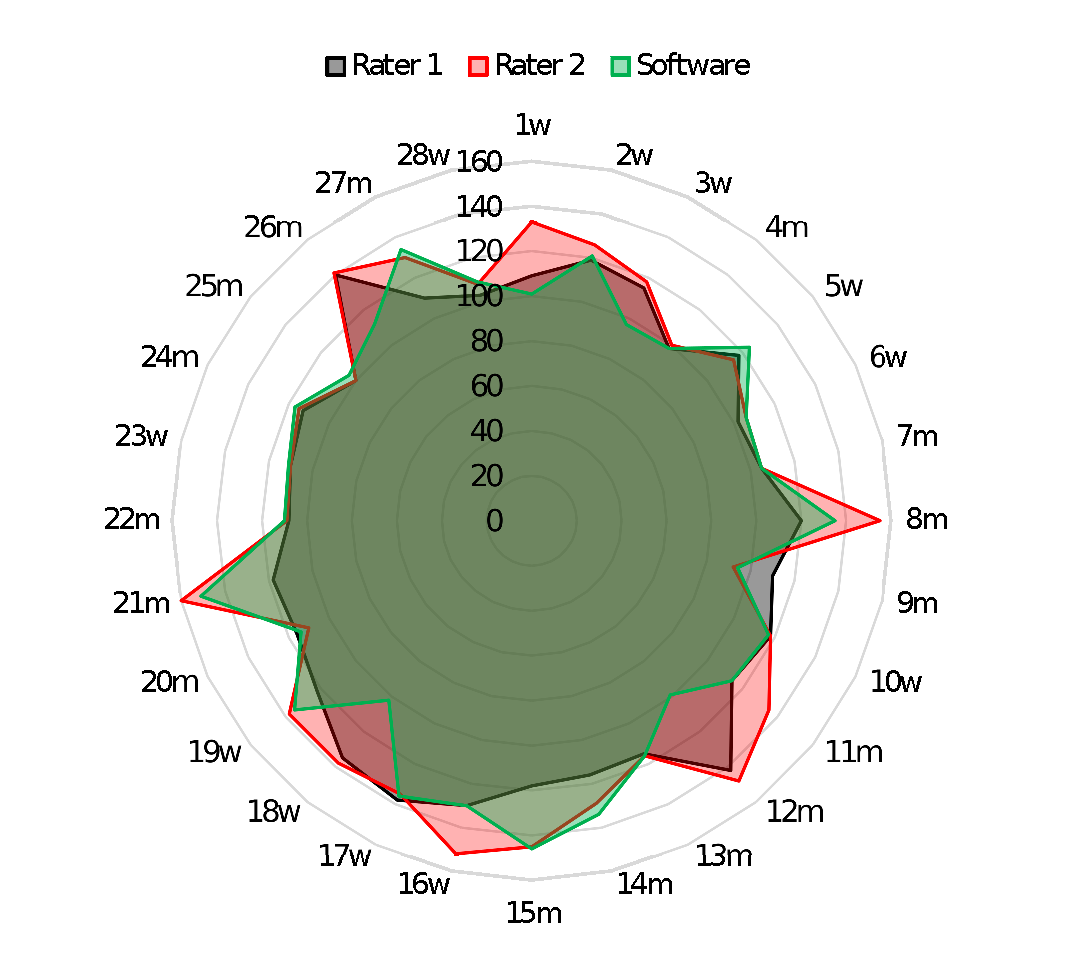
\includegraphics[scale=0.42]{Bilder/v-slope_net.eps}
			\subcaption[Vergleich der VT1-Bestimmungen durch V-Slope]{Vergleich der VT1-Bestimmungen durch V-Slope zwischen Ratern und Software; Intervall: \SIrange{0}{160}{\per\minute}}
			\label{subpic:pic1}
	\end{subfigure}%
	\hfil
	\begin{subfigure}[c]{0.45\textwidth}
		\centering
		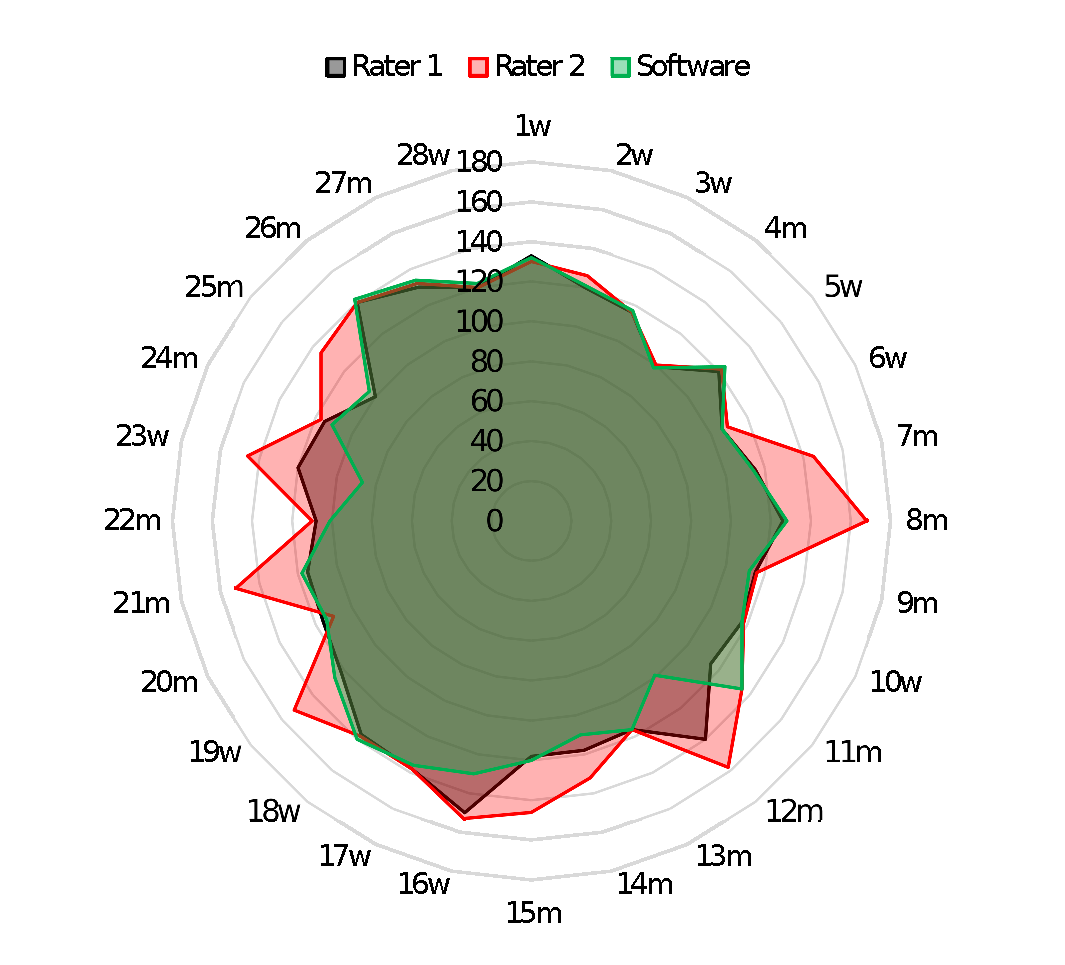
\includegraphics[scale=0.42]{Bilder/eqo2_net.eps}
			\subcaption[Vergleich der VT1-Bestimmungen durch das \gls{EQO2}]{Vergleich der VT1-Bestimmungen durch das \gls{EQO2} zwischen Ratern und Software; Intervall: \SIrange{0}{180}{\per\minute}}
			\label{subpic:pic2}
	\end{subfigure}
\caption[Grafische Darstellung der Übereinstimmung für die VT1]{Darstellung der Übereinstimmung zwischen Ratern und Software bei Bestimmung der VT1; Grau: Rater 1; Rot: Rater 2; Grün: Software; Kontrastierungen stellen Übereinstimmungen dar}
\label{pic:pic22}
\end{figure}
%
\begin{figure}[H]
	\centering
	%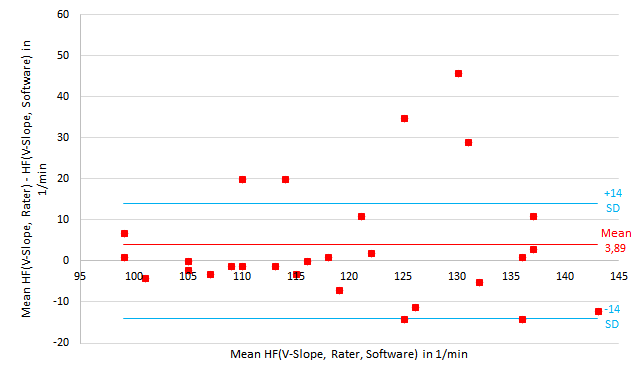
\includegraphics[scale=0.7]{Bilder/mean_vslope}
	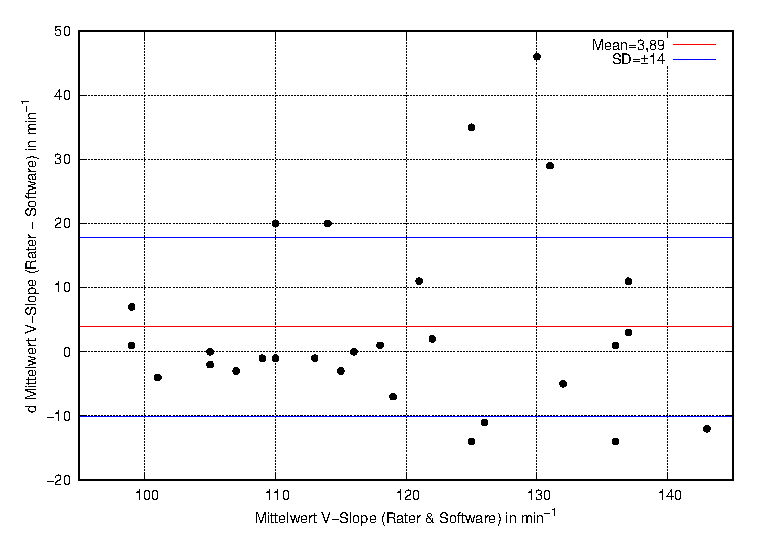
\includegraphics[scale=1]{Bilder/vslope.eps}
	\caption[Differenzen der V-Slope-Ergebnisse zwischen Ratern und Software]{Differenzen zwischen den Mittelwerten für die VT1 von Ratern und Software, die durch den V-Slope bestimmt wurden; rote Linie: Mean = Mittelwert der Rater-Software-Differenz, SD~=~Standardabweichung der Rater-Software-Ergebnisse}
	\label{pic:pic23}
\end{figure}
%
\begin{figure}[H]
	\centering
	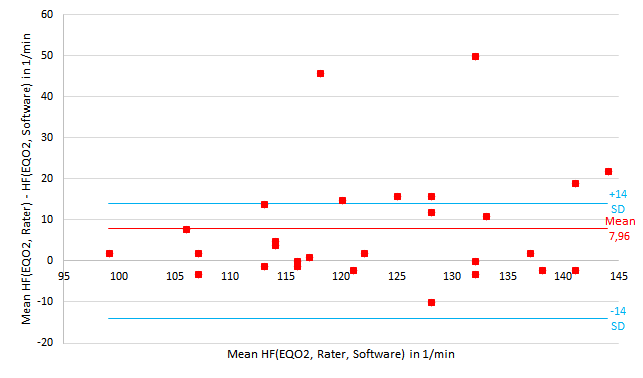
\includegraphics[scale=0.7]{Bilder/mean_eqo2}
	\caption[Differenzen der \gls{EQO2}-Ergebnisse zwischen Ratern und Software]{Differenzen zwischen den Mittelwerten für die VT1 von Ratern und Software, die durch das \gls{EQO2} bestimmt wurden; rote Linie: Mean = Mittelwert der Rater-Software-Differenz, SD~=~Standardabweichung der Rater-Software-Ergebnisse}
	\label{pic:pic24}
\end{figure}
%
Um zu analysieren, wie stark die Ergebnisse der Rater von denen der Software im Mittel differieren, wurden für beide Methoden Punktdiagramme erstellt, in denen die Differenzen aus den gemittelten VT1-Werten der Rater und der Software gegen die Gesamtmittelwerte für alle 28 Personen aufgetragen wurden. In Abb. \ref{pic:pic23} ist das Diagramm für die V-Slope-Methode abgebildet. Der Mittelwert der Differenzen zwischen Ratern und Software ist als rote Linie ins Diagramm einfügt. Die Werte für die VT1, die von Ratern und Software mittels V-Slope bestimmt wurden, unterscheiden sich durchschnittlich um $3,89$ $\pm$14 Schläge pro Minute.\\
Abb. \ref{pic:pic24} zeigt das Diagramm für die \gls{EQO2}-Methode mit den Differenzen zwischen Ratern und Software. Dort beträgt diese im Mittel \SI{7,98}{\per\minute} $\pm$14 \si{\per\minute}.
%
\subsection{Ergebnisse für VT2}
%
\begin{table}[H]
	\begin{center}
		\caption{Ergebnisse für die \gls{HF} in \si{\per\minute} bei VT2}
		\medskip
		\begin{tabulary}{\textwidth}{L@{\hspace{3em}} C C C C C C C}
			\toprule
			& \multicolumn{2}{c}{\textbf{Rater 1}} & \multicolumn{2}{c}{\textbf{Rater 2}} & \multicolumn{3}{c}{\textbf{Software}} \\
			\midrule
			ID & \gls{EQCO2} & \gls{VE}/\gls{VCO2} & \gls{EQCO2} & \gls{VE}/\gls{VCO2} & \gls{EQCO2} & \gls{VE}/\gls{VCO2} & RQ=1 \\
			\midrule
			\midrule
			1w & 163 & 162 & 160 & 163 & 162 & 162 & 166 \\
			2w & 161 & 159 & 161 & 173 & 161 & 177 & 155 \\
			3w & 143 & 145 & 142 & 145 & 155 & 143 & - \\
			4m & 143 & 145 & 140 & 140 & 144 & 144 & - \\
			5w & 158 & 158 & 160 & 171 & 172 & 182 & 177 \\
			6w & 130 & 130 & 158 & 159 & 159 & 159 & 154 \\
			7m & 150 & 150 & 150 & 162 & 151 & 161 & 166 \\
			8m & 163 & 163 & 180 & 170 & 169 & 180 & 192 \\
			9m & 160 & 160 & 160 & 161 & 160 & 128 & 173 \\
			10w & 161 & 161 & 162 & 162 & 164 & 164 & 152 \\
			11m & 149 & 160 & 160 & 164 & 162 & 162 & 172 \\
			12m & 165 & 168 & 168 & 169 & 159 & 159 & - \\
			13m & 150 & 149 & 151 & 150 & 160 & 150 & - \\
			14m & 158 & 162 & 166 & 164 & 165 & 165 & 171 \\
			15m & 186 & 185 & 187 & 187 & 188 & 187 & - \\
			16w & 170 & 170 & 169 & 169 & 171 & 185 & 181 \\
			17w & 160 & 159 & 159 & 178 & 172 & 187 & 155 \\
			18w & 170 & 172 & 168 & 169 & 170 & 170 & 180 \\
			19w & 158 & 159 & 156 & 158 & 157 & 168 & 156 \\
			20m & 162 & 163 & 169 & 169 & 168 & 168 & 189 \\
			21m & 150 & 155 & 152 & 182 & 163 & 183 & - \\
			22m & 130 & 140 & 151 & 152 & 141 & 141 & - \\
			23w & 145 & 143 & 149 & 145 & 158 & 146 & - \\
			24m & 160 & 159 & 160 & 159 & 160 & 170 & 113 \\
			25m & 137 & 137 & 152 & 153 & 144 & 153 & - \\
			26m & 158 & 158 & 157 & 158 & 157 & 157 & 168 \\
			27m & 158 & 158 & 175 & 178 & 159 & 188 & 191 \\
			28w & 212 & 213 & 208 & 210 & 213 & 213 & 209 \\
			\bottomrule
		\end{tabulary}
		\label{tab:tabelle6}
	\end{center}
\end{table}
%
In Tab. \ref{tab:tabelle6} sind die Werte für die \gls{HF} eingetragen, an denen Rater und Software die VT2 bestimmt haben. In dieser Tabelle wurde die Software-Spalte zusätzlich mit der Referenzmethode RQ~=~1 ergänzt. Bei 9 von 28 Testmessungen konnte mit dieser Methode keine VT2 bestimmt werden, da die betroffenen Probanden dauerhaft einen RQ~<~1 besaßen.
%
\begin{figure}[H]
	\centering
	\begin{subfigure}[c]{0.45\textwidth}
		\centering
		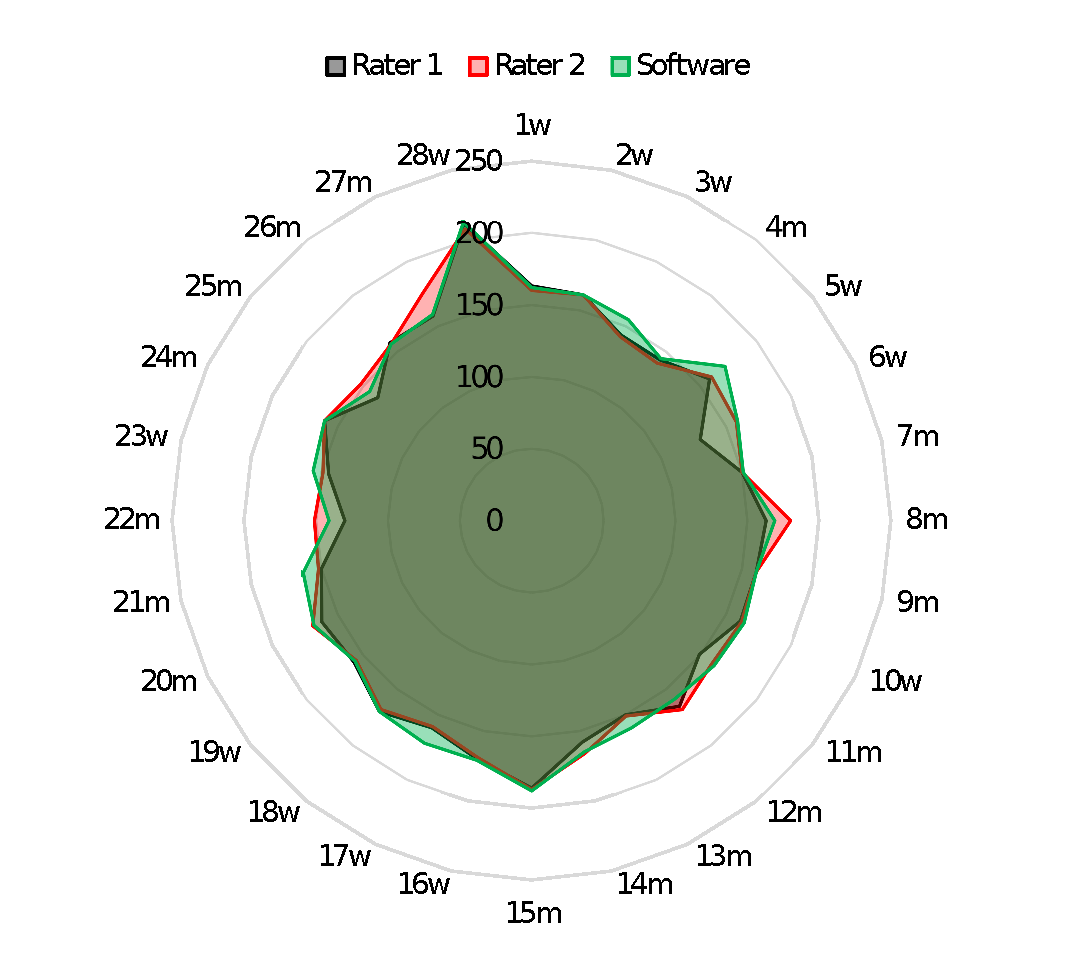
\includegraphics[scale=0.7]{Bilder/eqco2_net}
		\subcaption[Vergleich der VT2-Bestimmungen durch das \gls{EQCO2}]{Vergleich der VT2-Bestimmungen durch das \gls{EQCO2} zwischen Ratern und Software; Intervall: \SIrange{0}{250}{\per\minute}}
		\label{subpic:pic3}
	\end{subfigure}%
	\hfil
	\begin{subfigure}[c]{0.45\textwidth}
		\centering
		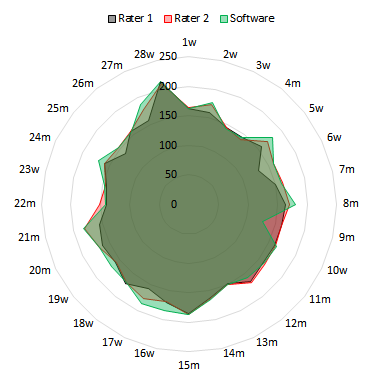
\includegraphics[scale=0.7]{Bilder/ve_vco2_net}
		\subcaption[Vergleich der VT2-Bestimmungen durch \gls{VE}/\gls{VCO2}]{Vergleich der VT2-Bestimmungen durch \gls{VE}/\gls{VCO2} zwischen Ratern und Software; Intervall: \SIrange{0}{250}{\per\minute}}
		\label{subpic:pic4}
	\end{subfigure}
	\caption[Grafische Darstellung der Übereinstimmung für die VT2]{Darstellung der Übereinstimmung zwischen Ratern und Software bei Bestimmung der VT2; Grau: Rater 1; Rot: Rater 2; Grün: Software; Kontrastierungen stellen Übereinstimmungen dar}
	\label{pic:pic25}
\end{figure}
%
Abb. \ref{pic:pic25} zeigt die Netzdiagramme für die VT2-Ergebnisse durch das \gls{EQCO2} und \gls{VE}/\gls{VCO2}.

\begin{figure}[H]
	\centering
	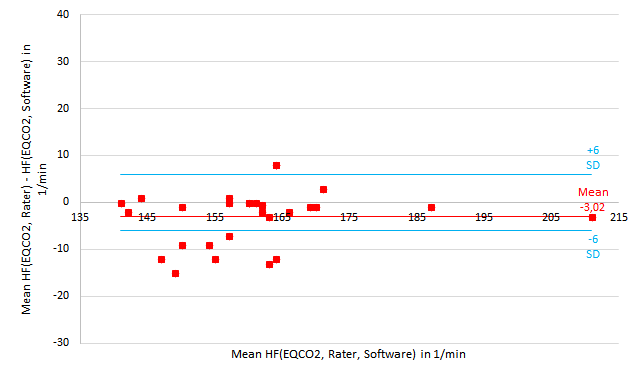
\includegraphics[scale=0.7]{Bilder/mean_eqco2}
	\caption[Differenzen der \gls{EQCO2}-Ergebnisse zwischen Ratern und Software]{Differenzen zwischen den Mittelwerten für die VT1 von Ratern und Software, die durch das \gls{EQCO2} bestimmt wurden; rote Linie: Mean = Mittelwert der Rater-Software-Differenz, SD~=~Standardabweichung der Rater-Software-Ergebnisse}
	\label{pic:pic26}
\end{figure}
%
In Abb. \ref{pic:pic26} ist die Streuung der \gls{EQCO2}-Methode dargestellt. Die durchschnittliche Differenz für die VT2, basierend auf dem \gls{EQCO2}, beträgt \SI{-3,02}{\per\minute} $\pm$6 \si{\per\minute}.
%
\begin{figure}[H]
	\centering
	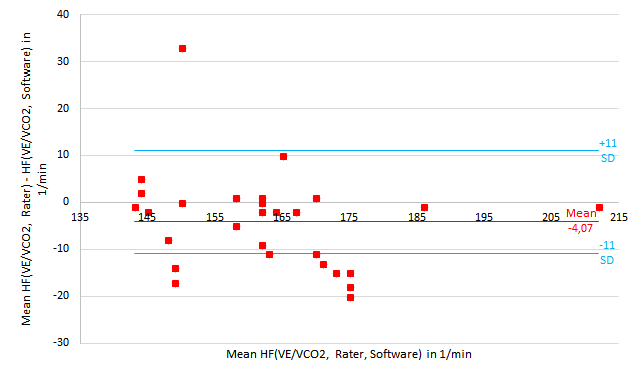
\includegraphics[scale=0.7]{Bilder/mean_vevco2}
	\caption[Differenzen der \gls{VE}/\gls{VCO2}-Ergebnisse zwischen Ratern und Software]{Differenzen zwischen den Mittelwerten für die VT1 von Ratern und Software, die durch \gls{VE}/\gls{VCO2} bestimmt wurden; rote Linie: Mean = Mittelwert der Rater-Software-Differenz, SD~=~Standardabweichung der Rater-Software-Ergebnisse}
	\label{pic:pic27}
\end{figure}
%
Abb. \ref{pic:pic27} zeigt die Abweichungen der Ergebnisse für \gls{VE}/\gls{VCO2}. Hier differieren Rater und Software um durchschnittlich \SI{-4,07}{\per\minute} bei einer \gls{SD} von $\pm$10 \si{\per\minute}.